
\documentclass[border=10pt]{standalone}
\usepackage{pgfplots}
\pgfplotsset{compat=1.18}
\begin{document}
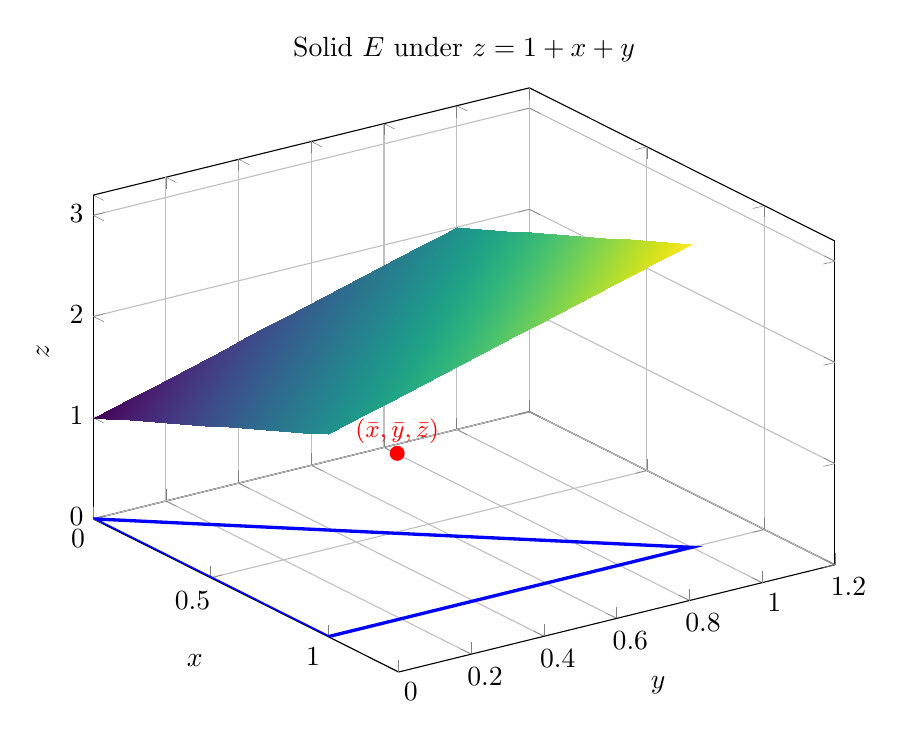
\begin{tikzpicture}
\begin{axis}[
    xlabel={$x$},
    ylabel={$y$},
    zlabel={$z$},
    title={Solid $E$ under $z=1+x+y$},
    xmin=0, xmax=1.3,
    ymin=0, ymax=1.2,
    zmin=0, zmax=3.2,
    grid=both,
    view={55}{30},
    samples=20,
    samples y=20,
    width=11cm, height=9cm
]
% Top surface (plane z = 1+x+y over region y <= sqrt(x))
\addplot3[
    surf,
    shader=interp,
    colormap/viridis,
    domain=0:1,
    y domain=0:1,
    restrict y to domain=0:1,
] {1 + x + y};
% Base boundary
\addplot3[blue, very thick] coordinates {(0,0,0) (1,0,0) (1,1,0) (0,0,0)};
% Center of mass point
\addplot3[
    only marks,
    mark=*,
    mark size=2.5pt,
    color=red,
] coordinates {(0.6474, 0.4177, 1.0325)};
\node[above, red] at (axis cs:0.6474, 0.4177, 1.0325) {\small $(\bar x, \bar y, \bar z)$};
\end{axis}
\end{tikzpicture}
\end{document}
